% Created 2018-07-05 Thu 17:29
% Intended LaTeX compiler: pdflatex
\documentclass[11pt]{article}
\usepackage[utf8]{inputenc}
\usepackage[T1]{fontenc}
\usepackage{graphicx}
\usepackage{grffile}
\usepackage{longtable}
\usepackage{wrapfig}
\usepackage{rotating}
\usepackage[normalem]{ulem}
\usepackage{amsmath}
\usepackage{textcomp}
\usepackage{amssymb}
\usepackage{capt-of}
\usepackage{hyperref}
\date{\today}
\title{Surface Excess Adsorption}
\hypersetup{
 pdfauthor={},
 pdftitle={Surface Excess Adsorption},
 pdfkeywords={},
 pdfsubject={},
 pdfcreator={Emacs 25.3.1 (Org mode 9.1.13)}, 
 pdflang={English}}
\begin{document}

\maketitle
\tableofcontents


\section{Definitions}
\label{sec:orgb397f16}

\section{Gibbs Dividing Surface}
\label{sec:org84c55be}
\begin{itemize}
\item the Gibbs Dividing Surface (GDS) is an arbirtary geometrical surface close to the adsorbing surface, with a precisely determined position
\begin{itemize}
\item it is assumed that adsorption takes place on the GDS
\end{itemize}
\end{itemize}

\begin{center}
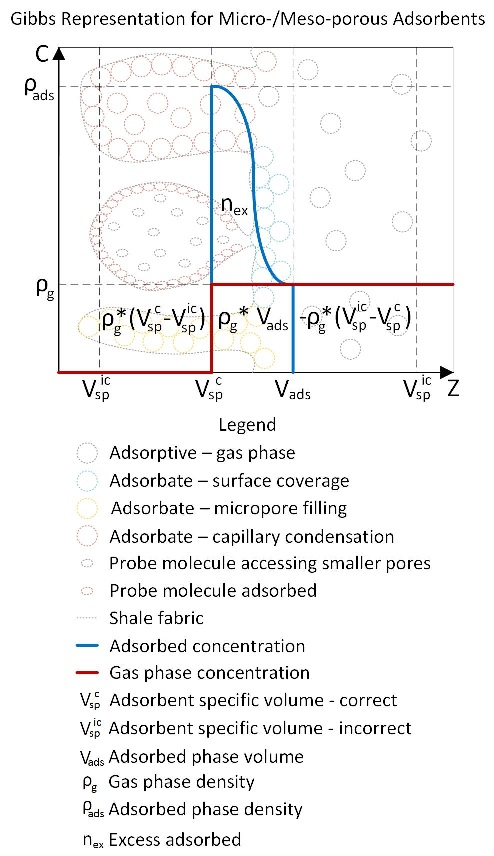
\includegraphics[width=.9\linewidth]{./gibbsrepresentation.jpg}
\end{center}
\cite{Rouquerol2016}

\subsection{Gibbs Exclusion Volume}
\label{sec:org98bd323}
\begin{itemize}
\item Gibbs Exclusion Volume \(V_{GDS}\) is the volume excluded by the GDS \cite{Rouquerol2016}
\begin{itemize}
\item by declaring such a variable, it is possible to exclude the uncertainties posed by void volume calculations from the surface excess amount
\item but this also means that the Gibbs Exclusion Volume must be reported along with the surface excess for it to be comparable
\end{itemize}
\end{itemize}

\subsection{Choice of the GDS}
\label{sec:org0fa453a}
\begin{itemize}
\item due to practical limitations are limited to the following \cite{Rouquerol2016}
\begin{itemize}
\item a probe-determined \(V_{GDS}\) close to the adsorbent specific volume \(V _i ^s\) for vapour adsorption below 1 bar
\item an arbirtray \(V_{GDS}\) of 0.5 cm3/g, which is close enough to the specific volume of many adsorbents
\item \(V_{GDS}\) of 0, yeilds net adsorption, particularly useful for evaluating gas storage
\end{itemize}
\end{itemize}
\begin{itemize}
\item \begin{center}
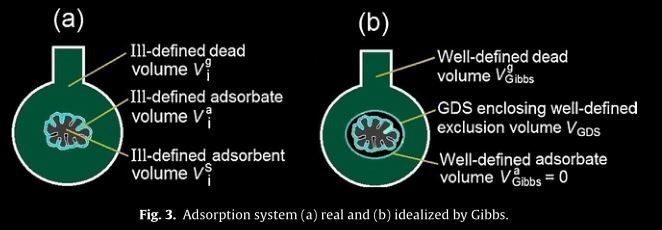
\includegraphics[width=.9\linewidth]{./gibbsrepresentation2.jpg}
\end{center}
\begin{itemize}
\item \cite{Rouquerol2016}
\end{itemize}
\end{itemize}

\section{Specific Volume of the Sample}
\label{sec:orga4d27fe}
\begin{itemize}
\item dead volume is the volume available to the gas phase \cite{Rouquerol2016}
\begin{itemize}
\item \(V _i ^g = V - ( V _i ^S + V _i ^a)\)
\item V is the sum of the volume of the empty adsorption bulb + the dosing volume up to the membrane of the pressure transducer
\begin{itemize}
\item \(V _i ^S\) is the adsorbent volume inaccessible to the molecules of the adsorptive i - the solid volume
\item \(V _i ^a\) is the volume of the adsorption space for the adsorptive i - the adsoptive volume
\end{itemize}
\item the usual method of void volume characterization is based on gas expansion using Helium, which is assumed to inert  
\begin{itemize}
\item it is now well known that He is, however, prone, to adsorption in micropores, leading to disproprtionately large void volumes and disproportionately small values for adsorption \cite{Rouquerol2016}
\item He absorption might also be appreciable for shales, especially at moisture equilibrated conditions
\item this effect maybe minimized by measuring dead volume at higher temperatures \cite{Rouquerol2016}
\item due to their dimensions, some of these pores might be inaccessible to larger adsorptive molecules.
\item these shortcomings can be in principle avoided by calculating void volume through gas expansion of the adsorptive molecules at a tempreature where adsorption is negligible, but this is not always practically possible \cite{Rouquerol2016}
\item in simulations, the dead volume is calculated using an r-distance surface, the volume limited by the probe-accessible surface - the connolly surface for spherical probes \cite{Rouquerol2016}
\item \begin{center}
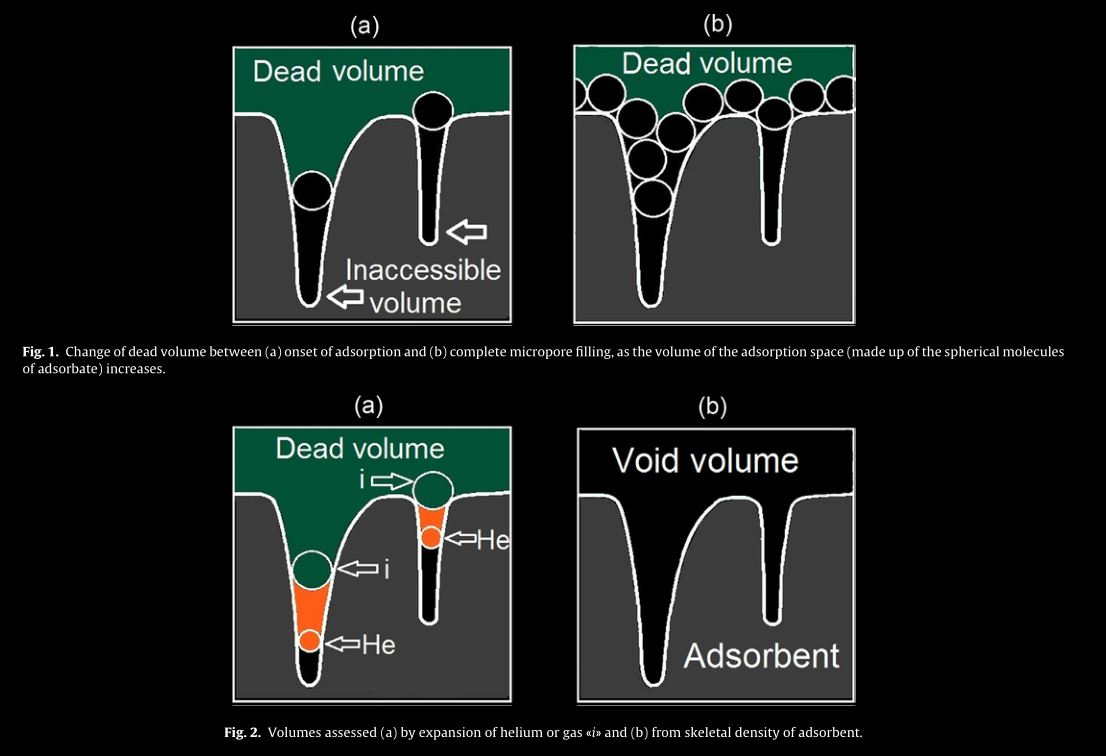
\includegraphics[width=.9\linewidth]{./voidvolumecalculation.jpg}
\end{center}
\end{itemize}
\end{itemize}
\end{itemize}

\section{Adsorption Space}
\label{sec:orgca36f5d}
\begin{itemize}
\item adsorption space is \(V _i ^a\) defined as the region in which the concentration of the adsorptive is higher compared to the bulk region or the gas phase \cite{Rouquerol2016}
\begin{itemize}
\item for the sake of simplicity, the adsorption space is often taken as 0 \cite{Rouquerol2016}
\item adsorbed phase volume, \(V _i ^a\) can either \cite{Rouquerol2016}
\begin{itemize}
\item be assumed to be equal to the micropore volume - with increasing density with loading, or
\item be assumed to have a constant density and increasing volume with loading
\end{itemize}
\end{itemize}

\item amount adsorbed is defined as the content of the adsorption space \cite{Rouquerol2016}
\end{itemize}

\section{Excess Adsorption}
\label{sec:org4968e0e}
\begin{itemize}
\item the resulting surface excess amount is given as: \cite{Rouquerol2016}
\begin{itemize}
\item \(n _\sigma = n - c^g (V - V _{GDS})\)
\begin{itemize}
\item n is the total adsorptive introduced into the system
\item cg is the final experimental concentration of the gas phase
\item \$V \_\{GDS\} is the gibbs exclusion volume that is decided by the coice of the GDS
\end{itemize}
\item it must be noted that most porous solids do not have a well defined adospriton surface, and hence the defenition of a Gibbs surface excess is not valid in most cases; however the concept of a surface excess amount can be an useful intermediate step in calculating  amount adsorbed.
\begin{itemize}
\item in adsorbates containing micropores less than 2 nm, dead volume of the gas phase is not very easy to measure.
\item a straight line or plane assumed to be the GDS cannot conicde with the more complex shape of the adsorptive-accessibe surface of the adsorbent.
\item it can be seen that for different arbitrary GDS positions, the excess adsorbed, \(n _{\sigma}\), calculated varies accordingly
\begin{itemize}
\item the space represented by the yellow rectangle is the portion of gas counted as gas
\item where \(n^a\) is the absolute adsorption
\item \(n ^{\sigma} = n^a - n^c - n^b\) for GDS-1
\item \(n ^{\sigma} = n^a - n^c\) for GDS-2
\item \(n ^{\sigma} = n^a + n^d\) for GDS-3
\end{itemize}
\item \begin{center}
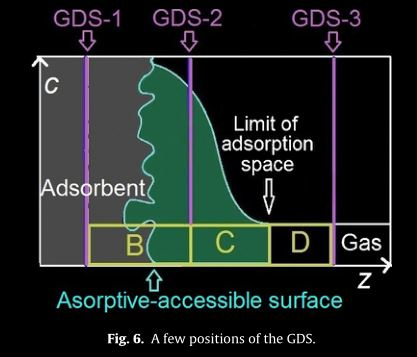
\includegraphics[width=.9\linewidth]{./gibbsrepresentation3.jpg}
\end{center}
\item \cite{Rouquerol2016}
\item \begin{center}
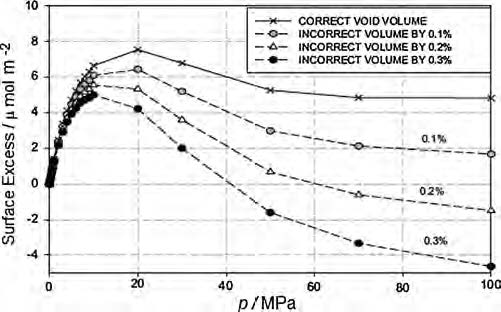
\includegraphics[width=.9\linewidth]{./Do2010.jpg}
\end{center}
\item \cite{Do2010}
\end{itemize}
\end{itemize}
\end{itemize}

\section{Net Adsorption}
\label{sec:orgce30d8e}
\begin{itemize}
\item net adsorption is calculated from a \(V_{GDS}\) of 0 \cite{Rouquerol2016}
\end{itemize}

\section{Absolute Adsorption}
\label{sec:org19c6c65}
\begin{itemize}
\item calculation of absolute adsorption requires knowledge of \cite{Rouquerol2016}
\begin{itemize}
\item \(V_{GDS}\) used to calculate \(n ^{\sigma}\)
\item gas law used the calculation of \(n ^{\sigma}\) to derive \(c ^g\)
\item specific inaccessible volume of the adsorbent \(V _i ^s\)
\item actual volume of the adsorbate \(V _i ^a\)
\end{itemize}
\item $$n ^a = n ^{\sigma} + c ^g V ^a + c ^g ( V _i ^S - V _{GDS} )$$ \cite{Rouquerol2016}
\end{itemize}

\subsection{Adsorbed Phase Volume / Density Correction Term}
\label{sec:org747e58a}
\begin{itemize}
\item \(c ^g V ^a\)
\item second term in the equation for absolute adsorption corrects the assumption of 0 adsorption volume in the Gibbs approach
\begin{itemize}
\item for sub-critical adsorption below 1 bar this term might be ignored
\item but this term becomes significant for adsorption above 10 bars and for super-critical adsorption
\end{itemize}
\end{itemize}

\subsection{Void Volume Correction Term}
\label{sec:org0bed323}
\begin{itemize}
\item \(c ^g ( V _i ^S - V _{GDS} )\)
\item thrid term accounts for the fact that GDS does not coincide with the adsorbing surface accessible to the adsorbate
\item can be ignored for low pressures due to low values fo \(c ^g\)
\begin{itemize}
\item for high pressure adsorption, due to an increased value of \(c ^g\), small errors in \(V _i ^s\) and \(V _i ^a\) lead to a significant error in amount adsorbed
\end{itemize}
\item for vapour adsorption at low pressures, below 1 bar, the difference between excess and absolute adsopriton is negligible.
\end{itemize}

\section{Equations of State}
\label{sec:orgfba7b83}
\begin{itemize}
\item the choice of equation of state, greatly affects calculated adsorption values
\begin{itemize}
\item whilst conventional equations such as Peng-Robinson and Redlich-Kwong are widely used, more precise EoS specific for individual gases have been proposed in the recent years.
\end{itemize}
\item it is challenging to find an EoS that adequately describes adsorption at near critical regions \cite{Siemons2007}
\end{itemize}

\section{Saturation Vapour Pressure}
\label{sec:orgf527146}
\begin{itemize}
\item saturation Vapour Pressure has been obtained through 
\begin{itemize}
\item a plot of log(vapour pressure) vs 1/T \cite{Clarkson1997}
\item from Chemical Engineering data books \cite{Lide2003}
\item from reduced Kirchoff equation \cite{Kapoor1989}
\begin{itemize}
\item \(P _s = P _c * exp[ \frac{T _{nbp}}{T _c} (\frac{ln P _c}{1 - T _{nbp}/T _c})(1 - \frac{T _c}{T}) ]\)
\end{itemize}
\end{itemize}
\item \cite{Clarkson1997} found that pseudo vapour pressures obtained from CRC handbook and Kirchoff equation provided the best results.
\end{itemize}

\section{Gravimetric Adsorption}
\label{sec:orgb89db3d}
\begin{itemize}
\item in gravimetric measurements, the effect of weight increase due to adsorption is reduced due to bouyancy, proportional to gas density \(\rho _i ^g\) \cite{Rouquerol2016}
\item excess adsorbed is given as:
\begin{itemize}
\item \(n ^{\sigma} = \frac{\Delta m + \Delta \rho _i ^g (V _{GDS} + V ^B)}{M_i}\)
\begin{itemize}
\item for gravimetric measurements, \(c ^g\) can be replaced by \(\rho _i ^g\) / M\(_{\text{i}}\)\$
\item \(\Delta m\) is the measured mass change
\item \(\rho _i ^g\) is the gas phase density
\item \(V _{GDS}\) is the Gibbs exclusion volume
\item \(V ^B\) is the volume of the gas phase
\item \(M _i\) is the molar mass of the adsorptive
\end{itemize}
\end{itemize}
\item absolute adsorbed is given as
\begin{itemize}
\item \(n ^a = n ^{\sigma} + (\frac{\Delta \rho _i ^g}{M _i}) V _i ^a + (\frac{\Delta \rho _i ^g}{M _i})*(V _i ^s - V_{GDS})\)
\begin{itemize}
\item \(V _i ^a\) is the volume of the adsorbed phase
\end{itemize}
\end{itemize}
\end{itemize}
\end{document}
